\documentclass{article}
\usepackage[dblblindworkshop]{neurips_2026}

\bibliographystyle{plainnat}
% \usepackage[preprint]{neurips_2026}          % for arXiv
\usepackage[utf8]{inputenc}
\usepackage[T1]{fontenc}
\usepackage{hyperref}
\usepackage{url}
\usepackage{booktabs}    % required by paper_tables.tex
\usepackage{multirow}    % required by paper_tables.tex
\usepackage{amsfonts}
\usepackage{amsmath}
\usepackage{nicefrac}
\usepackage{microtype}
\usepackage{xcolor}
\usepackage{graphicx}
\usepackage{tikz}
\usetikzlibrary{positioning, arrows.meta, shapes.geometric, calc, fit}



\graphicspath{{figs/}}
\newcommand{\todo}[1]{\textcolor{red}{[#1]}}


\title{IDM-JEPA: Semi-Supervised Action Inference via Inverse Dynamics
in Joint-Embedding Predictive Architectures}

\workshoptitle{World Models in Physical AI (NeurIPS 2026)}

\author{%
  \todo{Author} \\
  \todo{Affiliation} \\
  \texttt{\todo{email}} \\
}

\begin{document}

\maketitle

\begin{abstract}
Joint Embedding Predictive Architectures (JEPAs) offer a compelling framework for
learning world models directly in compact representation spaces. However, existing
methods remain dependent on dense, frame-by-frame action supervision, forcing them
to discard unlabeled transitions and reducing their ability to leverage
action-sparse or passive video datasets. In this work, we introduce IDM-JEPA, a
semi-supervised framework that enables stable end-to-end JEPA training on partially
labeled data by inferring missing control signals via an Inverse Dynamics Model. By
routing inferred latent action codes through the same encoder as ground-truth
actions, pseudo-actions and real actions become interchangeable during training and
downstream Model Predictive Control (MPC), at no cost to the planner, which searches
over recorded actions throughout. On the continuous PushT benchmark, IDM-JEPA reaches
$48.4\%$ planning success from $5\%$ action supervision, against $24.4\%$ for an
action-conditioned baseline trained on the labeled fraction alone under a matched
budget of gradient steps. The advantage is confined to the extreme-scarcity regime:
at an equal step budget the baseline reaches $72.4\%$ at $25\%$ supervision and
approaches full-data performance by $50\%$, leaving little headroom for any
semi-supervised method on a dataset of expert demonstrations whose unlabeled
transitions are largely redundant with the labeled ones. Enforcing
action-sensitivity through cycle-consistency on imagined transitions does not
substitute for grounding codes in recorded ones. Inferred actions substitute for
labels only where the unlabeled pool adds state coverage.
\end{abstract}

% =====================================================================
\section{Introduction}
\label{sec:intro}
Progress in embodied AI is bounded heavily by the availability of interaction data.
Latent world models, which learn dynamics in a compact representation space rather
than reconstructing pixels, allow planners to search over imagined futures
efficiently. Notably, Joint Embedding Predictive Architectures (JEPAs) like
LeWorldModel \citep{maes2026} pair a forward model with SIGReg regularization to achieve
state-of-the-art Model Predictive Control (MPC) on robotics benchmarks. Yet the
mechanism enabling this planning, conditioning the predictor on a frame-by-frame
action, creates a severe bottleneck: models are forced to discard unannotated
transitions, which often comprise a significant fraction of available video data.

While Inverse Dynamics Models (IDMs) and latent actions enable semi-supervised
learning in massive foundation models or reconstruction-heavy architectures
\cite{genie}, previous attempts to integrate IDMs into latent predictive
architectures have either used them on fully frozen encoders \cite{dynamo}, or
utilized them as alternative regularizers \cite{sensorimotor} rather than as a bridge for
semi-supervised learning. To the best of our knowledge, no framework currently
exists to safely impute missing actions during the end-to-end training of a JEPA
without destabilizing its latent geometry. To eliminate this strict need for dense
supervision, we propose IDM-JEPA, a framework integrating an IDM that infers
missing latent action codes from consecutive states. By routing these
pseudo-actions through the standard action encoder, latent and ground-truth actions
occupy a shared space, making them interchangeable. This simulates complete action
coverage during training and downstream MPC. A teacher-forcing loss on labeled data
grounds the IDM, while the dimensionality constraint of the action code prevents
the predictor from trivially memorizing the future state.

On the continuous PushT benchmark, IDM-JEPA achieves $48.4\%$ planning success with
only $5\%$ action supervision, roughly twice the $24.4\%$ reached by an
action-conditioned baseline given the same number of gradient steps on the labeled
fraction alone. This advantage does not persist as supervision increases. Trained to
an equal step budget, the baseline reaches $72.4\%$ at $25\%$ supervision and
$80.8\%$ at $50\%$, within noise of full-data performance, leaving no headroom for
imputation to exploit. Interpolating the baseline curve. We
attribute the gap between these two figures to the redundancy of expert
demonstrations, under which a small labeled subset already covers most of the state
manifold, and to the difficulty of the inverse problem at contact, where PushT's
dynamics are discontinuous in the action.


\paragraph{Contributions.}
\begin{itemize}
  \item \textbf{Architecture}: We propose IDM-JEPA, a framework combining an inverse
    dynamics objective with SIGReg anti-collapse regularization to enable stable,
    end-to-end semi-supervised JEPA training for policy based tasks.
  \item \textbf{Evaluation}: We benchmark IDM-JEPA on the continuous PushT task
    across label fractions (0\%--100\%), state composition modes (Delta vs.\
    Concatenation), and masking granularity (Per-transition vs.\ Per-episode).
 
\end{itemize}

% =====================================================================
\section{Method}
\label{sec:method}

\paragraph{Overview.}
IDM-JEPA extends an action-conditioned latent world model with an inverse
dynamics model (IDM) $g_\phi$ that maps a pair of consecutive latents to a
\emph{latent action code} of the width of a recorded action
(Fig.~\ref{fig:architecture}). The code substitutes for the action wherever a
label is missing, and an unlabeled transition contributes a gradient to the
predictor and the encoder. At test time the planner searches over recorded
actions alone and is unchanged from the baseline. The method rests on two
design choices, a width constraint under which codes and actions enter the
predictor through a shared action encoder (Eq.~\ref{eq:idm}), and an
action-teacher term anchoring codes to the recorded action space on the labeled
fraction (Eq.~\ref{eq:objective}).

\paragraph{Dataset and setting.}
We study offline, reward-free learning from a dataset of episodes sub-sampled at a
stride of $K$ environment steps, observed only through images
$o \in \mathcal{O}$. The action signal attached to a frame is the block of $K$ raw
controls executed over that interval,
$a_t = (u_{Kt}, \dots, u_{Kt+K-1}) \in \mathbb{R}^{K d_{\mathrm{raw}}}$.
A mask $m_t \in \{0,1\}^{K}$ records which raw controls in block $t$ were observed,
and the labeled fraction $\rho = \mathbb{E}[m_t]$ gives the ratio of labeled
transitions in the dataset. A task is given at test time as a goal observation
$o_g$ and solved by model predictive control (MPC) over the learned latents, under
a success criterion internal to the environment (App.~\ref{app:setting}).

\paragraph{Notation and base architecture.}
A standard action-conditioned world model comprises an encoder
$z_t = f_\theta(o_t)$ mapping $\mathcal{O} \to \mathbb{R}^{d}$, an action encoder
$h_\psi : \mathbb{R}^{K d_{\mathrm{raw}}} \to \mathbb{R}^{d}$, and a predictor
$\hat z_{t+1} = p_\xi(z_{t-H+1:t},\, h_\psi(\tilde a_{t-H+1:t}))$ over a history of
$H$ frames, with latent width $d$.

\paragraph{Two gaps in action-conditioned latent world models.}
The action-conditioned objective of a JEPA world model is defined only where an
action was recorded:
\begin{equation}
  \mathcal{L}^{\mathrm{AC}}
  \;=\;
  \mathbb{E}_t\Bigl[\,
    \mathbf{1}\{m_t = \mathbf{1}\}\,
    \bigl\lVert
      p_\xi\bigl(z_{t-H+1:t},\, h_\psi(a_{t-H+1:t})\bigr) - z_{t+1}
    \bigr\rVert^{2}
  \Bigr]
  \;+\;
  \lambda_{\mathrm{sig}}\, \mathrm{SIGReg}\bigl(\{z\}\bigr).
  \label{eq:ac}
\end{equation}
Two properties of this objective bound what can be learned. First, an unlabeled
transition contributes no gradient to any parameter: for a block with
$m_t = \mathbf{0}$ the indicator annihilates the gradient with respect to the
action pathway $h_\psi$, the encoder $f_\theta$ and the predictor $p_\xi$ alike,
and the effective training set shrinks in proportion to $\rho$. Second, a
substitute action must be admissible to the planner. MPC searches over $h_\psi(a)$
for $a \in \mathcal{A}$, so a separately parameterized conditioning channel
carrying a free latent variable on unlabeled steps would learn dynamics outside the
reach of $\mathcal{A}$ and therefore unavailable to the planner. A substitute
action must share the input space the planner searches; Eq.~\ref{eq:idm} constrains
the codomain of $g_\phi$ accordingly.

\paragraph{Inverse dynamics model and mixed supervision.}
$g_\phi$ recovers the action that carried the system between two consecutive
latents. It is a small MLP applied to a single composition of the pair,
\begin{equation}
  \begin{gathered}
    g_\phi : \mathbb{R}^{d} \times \mathbb{R}^{d} \to \mathbb{R}^{K d_{\mathrm{raw}}},
    \qquad
    \hat{a}_t = g_\phi(z_t, z_{t+1}) = \operatorname{MLP}_\phi\bigl(\iota(z_t, z_{t+1})\bigr),
    \\[4pt]
    \iota(z_t, z_{t+1}) =
    \begin{cases}
      z_{t+1} - z_t & (\emph{delta}),\\[2pt]
      \bigl[\, z_t,\; z_{t+1} \,\bigr] & (\emph{concat}),
    \end{cases}
  \end{gathered}
  \label{eq:idm}
\end{equation}
where $\iota$ is the only difference between the two input modes we compare.
The map has three properties. (i) \emph{Interchangeability}. The output width
equals the action width $K d_{\mathrm{raw}}$, so
$\operatorname{cod}(g_\phi) = \operatorname{dom}(h_\psi)$. A latent code is a
syntactically valid action and enters the predictor through the same action encoder
as a recorded action.
(ii) \emph{Grounding}. $\mathcal{L}_{\mathrm{act}}$ pulls a latent code toward the
action a labeled transition would have carried, rather than toward a code
selected only for its predictive value. (iii) \emph{Bottleneck}. The width
constraint caps the channel at $K d_{\mathrm{raw}}$ scalars per transition and
bounds what $\hat{a}_t$ alone can carry about $z_{t+1}$.

Labeled and unlabeled components are combined into a single action fed to the
predictor,
\begin{equation}
  \tilde a_t \;=\; m_t \odot a_t \;+\; (1 - m_t) \odot \hat{a}_t ,
  \label{eq:mix}
\end{equation}
with $m_t$ broadcast over the $d_{\mathrm{raw}}$ components of each raw control.
Every transition contributes to training. At fixed $\rho$ we compare two
allocations of the label budget: \emph{per-transition}, where the mask is drawn
independently for each $K$-block, and \emph{per-episode}, where whole trajectories
are either fully labeled or fully unlabeled.

\paragraph{Training objective.}
The model is trained end to end on a single objective,
\begin{equation}
  \mathcal{L}
  \;=\;
  \underbrace{\bigl\lVert \hat z_{t+1} - z_{t+1} \bigr\rVert^{2}}_{\textstyle \mathcal{L}_{\mathrm{pred}}}
  \;+\;
  \lambda_{\mathrm{sig}}\,
  \underbrace{\mathrm{SIGReg}\bigl(\{z\}\bigr)}_{\textstyle \mathcal{L}_{\mathrm{sig}}}
  \;+\;
  \lambda_{\mathrm{act}}\,
  \underbrace{\frac{\sum_{k} m_t^{k}\,\bigl(\hat{a}_t^{k} - a_t^{k}\bigr)^{2}}
                   {\sum_{k} m_t^{k}}}_{\textstyle \mathcal{L}_{\mathrm{act}}}.
  \label{eq:objective}
\end{equation}
$\mathcal{L}_{\mathrm{pred}}$ is a next-state prediction loss term, taken against
the encoder's own output. The target $z_{t+1}$ is produced by the same encoder as
the context and is left attached, with the gradient reaching the prediction and the
target alike. $\mathcal{L}_{\mathrm{sig}}$ is a SIGReg anti-collapse loss term
\cite{lejepa}, penalizing departure of the embedding distribution from an isotropic
Gaussian along random projections. $\mathcal{L}_{\mathrm{act}}$ is a
teacher-forcing action-alignment loss term, averaged over labeled components.

\paragraph{Gradient flow.}
The model contains no stop-gradients, detached targets or target network;
Table~\ref{tab:gradflow} summarizes which modules each term updates in one backward
pass. $\mathcal{L}_{\mathrm{act}}$ anchors the IDM output to the recorded action
space on the labeled fraction $\rho$ and $\mathcal{L}_{\mathrm{pred}}$ shapes it on
the remaining $1-\rho$, both also reaching the encoder, so supervision propagates
from the labeled fraction to the unlabeled one through the shared parameters rather
than through the data. At $\rho = 1$ the objective reduces to the
action-conditioned baseline plus $\mathcal{L}_{\mathrm{act}}$; at $\rho = 0$ the
action channel is unconstrained and $\mathcal{L}_{\mathrm{act}}$ vanishes.

\begin{table}[t]
  \centering
  \small
  \caption{Direct gradient flow from each loss term in one backward pass.}
  \label{tab:gradflow}
  \begin{tabular}{lcccc}
    \toprule
    & Encoder $f_\theta$ & Action enc.\ $h_\psi$ & Predictor $p_\xi$ & IDM $g_\phi$ \\
    \midrule
    $\mathcal{L}_{\mathrm{pred}}$ & $\checkmark$ & $\checkmark$ & $\checkmark$ & $\checkmark^{\dagger}$ \\
    $\mathcal{L}_{\mathrm{sig}}$  & $\checkmark$ &              &              & \\
    $\mathcal{L}_{\mathrm{act}}$  & $\checkmark$ &              &              & $\checkmark$ \\
    \bottomrule
  \end{tabular}
  \\[2pt]
  {\footnotesize $^{\dagger}$ through the components with $m_t^{k} = 0$ only.}
\end{table}

\paragraph{Cycle-JEPA.}
We additionally test whether action-sensitivity enforced on \emph{imagined}
transitions substitutes for grounding codes in recorded ones. For each context
latent $z_t$, an action $a$ is drawn uniformly from the labeled actions of the
minibatch and applied to $z_t$; the predictor produces an imagined successor, which
$g_\phi$ then inverts:
\begin{equation}
  \hat z^{\,a}_{t+1} = p_\xi\bigl(z_t,\, h_\psi(a)\bigr),
  \qquad
  \mathcal{L}_{\mathrm{cyc}}
    = \bigl\lVert g_\phi\bigl(z_t,\, \hat z^{\,a}_{t+1}\bigr) - a \bigr\rVert^{2}.
  \label{eq:cycle}
\end{equation}
The term enters Eq.~\ref{eq:objective} with weight
$\lambda_{\mathrm{cyc}} = \lambda_{\mathrm{act}}$, retaining
$\mathcal{L}_{\mathrm{act}}$, and its gradients reach the predictor, penalizing
forward models whose imagined successors are insensitive to the conditioning
action. The counterfactual pairing permits the constraint at every latent while
restricting the action distribution to the labeled subset (App.~\ref{app:impl}).

\begin{figure}
  \centering
  \includegraphics[width=1\linewidth]{idm_architecture_diagram_horizontal.pdf}
  \caption{\textbf{Overview of the IDM-JEPA architecture.} A shared encoder maps
    consecutive observations $o_t$ and $o_{t+1}$ to latents $z_t$ and $z_{t+1}$,
    each regularized by SIGReg. A composition function combines the two latents,
    and an inverse model predicts the action $\hat{a}_t$ that explains the
    transition, supervised by the recorded action $a_t$. The action selection
    module passes either the predicted or the recorded action (teacher forcing)
    to the action encoder, whose embedding is fed together with $z_t$ to the
    forward model to obtain $\hat{z}_{t+1}$. The forward model is trained to
    match the encoder's own $z_{t+1}$ under an MSE loss. Dashed red arrows
    denote training signals; all other arrows denote the forward pass.}
  \label{fig:architecture}
\end{figure}

% =====================================================================
\section{Experimental setup}
\label{sec:setup}

\paragraph{Environment.}
All experiments use PushT (\texttt{swm/PushT-v1}), a continuous 2-D task in which
an agent pushes a T-shaped block to a target pose. Contact makes the dynamics
discontinuous in the action, so on the subset of transitions where the pusher meets
the block, recovering a control signal from a pair of observations is not merely a
matter of reading off ego-motion --- a stringent test of whether inferred codes
capture interaction with the object rather than movement of the agent alone. Raw
controls are $d_{\mathrm{raw}} = 2$ and we sub-sample at stride $K = 5$, so a
recorded action block lies in $\mathbb{R}^{10}$.

\paragraph{Dataset and supervision.}
We train on 20 000 expert demonstrations with mean episode length 196, holding out
$10\%$ for validation. Label scarcity is simulated by masking recorded actions
rather than by collecting unlabeled data, so unlabeled transitions are
in-distribution; this isolates the effect of missing annotation from the
distribution shift that accompanies genuinely passive data, and we return to the
distinction in Sec.~\ref{sec:conclusion}. Masks are drawn deterministically from
the transition index, so a given labeled fraction selects an identical subset
across every arm. Under per-transition supervision the mask applies to individual
$K$-step blocks; under per-episode supervision, to whole episodes.

\paragraph{Arms.}
We evaluate five arms at each labeled fraction. \emph{IDM-JEPA (delta)} and
\emph{IDM-JEPA (concat)} differ only in $\iota$ (Eq.~\ref{eq:idm}).
\emph{LeWM} is the action-conditioned baseline of Eq.~\ref{eq:ac}, trained on the
labeled fraction alone with unlabeled transitions discarded. \emph{Cycle-JEPA}
adds Eq.~\ref{eq:cycle} to the concat variant. \emph{Random} samples action
sequences uniformly from $\mathcal{A}$ and fixes the floor of the success scale.
All learned arms share encoder, predictor and optimizer settings and are trained to
the same number of \emph{gradient steps} (see \emph{Training budget} below),
differing only in which loss terms are active and, for LeWM, in the transitions
retained.

\paragraph{Architecture.}
We adopt the LeWM encoder and predictor \citep{sobal2025lewm}: a ViT-Tiny encoder trained
from scratch whose CLS token is projected to $z \in \mathbb{R}^{d}$ with
$d = 192$, and a $6$-layer autoregressive transformer predictor over a history of
$H = 3$ frames. Our only architectural addition is $g_\phi$, an MLP with two
GELU hidden layers of width $512$ mapping $\mathbb{R}^{d}$ (delta) or
$\mathbb{R}^{2d}$ (concat) to $\mathbb{R}^{10}$. Loss weights are $\lambda_{\mathrm{sig}} = 0.09$ and
$\lambda_{\mathrm{act}} = 0.1$; parameter counts, action injection and remaining
optimizer settings are in App.~\ref{app:impl}.

\paragraph{Planning.}
We perform goal-conditioned trajectory optimization in latent space following
LeWM \citep{sobal2025lewm}. Given a current observation $o_1$ and a goal observation $o_g$,
both are encoded and the predictor is rolled out autoregressively from
$\hat z_1 = z_1$ under a candidate sequence of $H_{\mathrm{plan}} = 5$ action
blocks. Candidates are scored by terminal goal-matching cost
$C(a_{1:H_{\mathrm{plan}}}) = \lVert \hat z_{H_{\mathrm{plan}}+1} - z_g \rVert_2^2$
and minimized with the Cross-Entropy Method \citep{rubinstein1999cem}, which at
each iteration samples action
sequences from a Gaussian, scores them by latent rollout, and refits the sampling
distribution to the top-scoring fraction (hyperparameters in App.~\ref{app:impl}).
Because rollout error accumulates with horizon, CEM is wrapped in a
receding-horizon loop that executes the first $E = 5$ blocks before
re-encoding and replanning; with $E = H_{\mathrm{plan}}$ the whole optimized
sequence is executed and the model is re-encoded once per plan. Episodes are given a budget of 50 environment
steps, with goals placed 25 steps ahead of the initial state. All learned
modules are frozen; only the action sequence is optimized. The planner
searches over $\mathcal{A}$ at test time.


\paragraph{Evaluation protocol.}
Each cell runs $50$ episodes over five evaluation seeds ($n = 250$); we report
mean\,$\pm$\,s.e.m.\ over seeds. Success is the criterion supplied by the
\texttt{swm/PushT-v1} environment and is never optimized directly: the planner
minimizes latent goal-matching cost and the environment scores the resulting
trajectory. \todo{state the rule verbatim from stable\_worldmodel's PushT
environment (coverage threshold and whether it is evaluated at the final step or
at any step); it could not be read off the result files, which record only the
boolean outcome.}

% =====================================================================
\section{Results}
\label{sec:results}

% TODO before submission: regenerate the left panel from the compute-matched
% baseline, plotting both the epoch-8 and step-matched curves.
\begin{figure}[t]
  \centering
  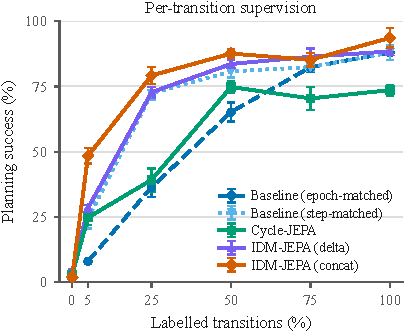
\includegraphics[width=0.48\linewidth]{planning_accuracy_vs_label_fraction_per_transition.pdf}
  \hfill
  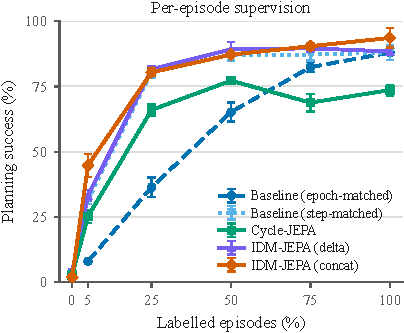
\includegraphics[width=0.48\linewidth]{planning_accuracy_vs_label_fraction_per_episode}
  \caption{\textbf{Planning curves.}
           Planning success on PushT vs.\ labeled fraction, per-transition (left)
           and per-episode (right). IDM-JEPA (concat) reaches $48.4\%$ at $5\%$ supervision
           against the compute-matched baseline's $24.4\%$; the baseline recovers
           to $72.4\%$ by $25\%$ supervision and saturates thereafter. The
           baseline is drawn under both budgets: epoch-matched (epoch~8, as
           every other arm) and step-matched (epoch $8/\rho$, see
           \emph{Training budget}); only the latter is a compute-matched
           comparison. Mean $\pm$ s.e.m.\ over five evaluation
           seeds ($n{=}250$ episodes per cell); one training seed per arm.}
  \label{fig:planning}
\end{figure}

\begin{table}[t]
  \centering
  \small
  \caption{Planning success (\%) on PushT, per-transition masking. The baseline
    is shown under both budgets; $\Delta$ is the correction from epoch-matching to
    step-matching. Mean $\pm$ s.e.m.\ over five evaluation seeds
    ($n = 250$), except where noted.}
  \label{tab:budget}
  \begin{tabular}{lcccc}
    \toprule
    $\rho$ & Baseline, epoch $8$ & Baseline, matched steps & $\Delta$ & IDM-JEPA (concat) \\
    \midrule
    $0.05$ & $8.0 \pm 0.9$  & $24.4 \pm 3.8$ (ep.\ $160$) & $+16.4$ & $48.4 \pm 2.9$ \\
    $0.25$ & $36.4 \pm 3.8$ & $72.4 \pm 2.3$ (ep.\ $32$)  & $+36.0$ & $79.2 \pm 3.3$ \\
    $0.50$ & $65.2 \pm 3.6$ & $80.8 \pm 2.3$ (ep.\ $16$)  & $+15.6$ & $87.6 \pm 1.7$ \\
    $0.75$ & $82.4 \pm 1.9$ & $82.4 \pm 1.3$ (ep.\ $11$) & $-2.4$ & $85.2 \pm 2.6$ \\
    $1.00$ & \multicolumn{2}{c}{$88.0 \pm 2.8$} & --- & $93.6 \pm 3.7$ \\
    \bottomrule
  \end{tabular}
  \\[2pt]
\end{table}


\subsection{Planning results}
\label{sec:results-planning}


\paragraph{The baseline saturates by $\rho = 0.5$.}
Given equal steps, the baseline reaches $72.4 \pm 2.3$ at $\rho = 0.25$ and
$80.8 \pm 2.3$ at $\rho = 0.50$, within noise of its $\rho = 0.75$ value of
$82.4 \pm 1.3$.
Replaying a labeled subset of half the transitions therefore recovers essentially all
of full-data planning performance on this dataset. Any method acting only on
unlabeled transitions is bounded above by the full-data result, leaving at most a few
points of headroom above $\rho \approx 0.25$, which the intervals cannot resolve.


\paragraph{IDM-JEPA doubles planning success in the extreme-scarcity regime.}
At $\rho = 0.05$, IDM-JEPA (concat) reaches $48.4 \pm 2.9$ against the
compute-matched baseline's $24.4 \pm 3.8$. The $24.0$-point difference is $5.0$
pooled s.e.m., the only separation in the sweep that evaluation noise cannot
plausibly explain; every arm sits far above the $\rho = 0$ floor of
$2.0$--$4.0$, where $\mathcal{L}_{\mathrm{act}}$ vanishes and the code space is
ungrounded. The composition function matters at this fraction and only at this
fraction: concat reaches $48.4 \pm 2.9$ where delta reaches $28.4 \pm 1.2$,
while by $\rho \ge 0.50$ the two are indistinguishable ($87.6 \pm 1.7$
vs.\ $83.6 \pm 1.6$). Delta can express the action only as an additive
correction in latent space, whereas concat receives $z_t$ and $z_{t+1}$
separately and can condition on absolute position --- which is what PushT
demands, since the effect of a control depends on the contact geometry between
pusher and block and not on displacement alone. Notably, delta at $\rho = 0.05$
($28.4 \pm 1.2$) is itself within noise of the compute-matched baseline, so the
entire measured advantage of the method at extreme scarcity is carried by the
concat composition. Under per-episode masking the same ordering holds with
concat at $44.8 \pm 4.4$, so the result does not depend on labels being
scattered across episodes.


\paragraph{Cycle-consistency does not substitute for grounding.}
Cycle-JEPA never beats the baseline above $\rho = 0.05$ and is worse than it
almost everywhere: $39.2 \pm 4.4$ against $72.4 \pm 2.3$ at $\rho = 0.25$,
$70.4 \pm 4.4$ against $82.4 \pm 1.3$ at $\rho = 0.75$, and $73.6 \pm 2.0$
against $88.0 \pm 2.8$ at full supervision, a $14.4$-point deficit at $4.2$
pooled s.e.m. All full-data arms were trained on identical schedules and are
unaffected by the budget correction, so this comparison is internally
compute-matched and the deficit is attributable to the objective. The one-step
latent error tells the same story from the other side: Cycle-JEPA is the only
arm whose prediction error fails to improve with supervision, sitting at
$2.26 \times 10^{-2}$ at $\rho = 1$ against $0.78$ for both the baseline and
IDM-JEPA (concat) (Table~\ref{tab:next-state}).

The probes locate the failure, and it is not a failure of grounding. At
$\rho = 1$ Cycle-JEPA's codes decode the recorded action as well as
IDM-JEPA's do ($c \to a$ ridge $R^2$ of $0.888$ against $0.891$), and its
encoder probes are indistinguishable from every other arm's. The codes are
therefore correct and the representation is intact; what degrades is the
forward model, which is asked to make imagined successors invertible under an
action drawn independently of the transition that produced $z_t$. Enforcing
action-sensitivity on counterfactual pairs buys nothing the action-teacher term
does not already supply, and costs accuracy on the real ones. Grounding codes
in recorded transitions, rather than consistency on imagined ones, is what the
method needs.

% =====================================================================
\section{Related work}
\label{sec:related}

\paragraph{Latent world models for planning.}
World models that predict in a learned representation space rather than in pixels
avoid spending capacity on visually salient but control-irrelevant detail, and allow
a planner to roll out candidate action sequences cheaply. Joint-Embedding Predictive
Architectures \citep{lecun2022path, assran2023ijepa, bardes2024vjepa} formalize
this by training a predictor to match the
embedding of a future observation produced by the same encoder, with an explicit
regularizer preventing the representational collapse that the objective otherwise
admits. LeWM \citep{sobal2025lewm} instantiates this for control, pairing an
action-conditioned predictor with SIGReg and planning by Cross-Entropy Method over
latent rollouts; V-JEPA~2 \citep{assran2025vjepa2} scales the same recipe to
robot manipulation, and both depend on densely recorded actions. Latent-space
model-predictive control is of course not confined to JEPAs
\citep{hafner2021dreamerv2, hansen2024tdmpc2}; what distinguishes this family is
that the prediction target is the encoder's own output rather than a
reconstruction, which is precisely what makes the action channel the only route
by which control information enters the representation.

\paragraph{Inverse dynamics and latent actions.}
Recovering the action that connects two observations is a long-standing device for
extracting control signal from unlabeled video. VPT \citep{baker2022vpt} trains an
inverse dynamics model on a small labeled set and uses it to pseudo-label a large
unlabeled corpus, which is then consumed by an otherwise standard supervised
pipeline. LAPO \citep{schmidt2024lapo} and Genie \citep{bruce2024genie} instead
learn a discrete or continuous latent action space with no recorded actions at all,
recovering a controllable interface post hoc. Both lines operate either offline from
the world model, as a separate pseudo-labeling stage, or on a frozen encoder. The
end-to-end case differs in that the IDM's inputs are themselves being learned: the
code $\hat a_t$ is a function of representations that the same objective is
simultaneously reshaping.

\paragraph{Evaluating semi-supervised methods.}
The compute-matched baseline finding is an instance of a documented pattern.
\citet{oliver2018realistic} reimplemented a range of deep semi-supervised algorithms
under a unified protocol and found that the performance of simple supervised
baselines that discard unlabeled data is often underreported, and that the gap
between those baselines and semi-supervised methods narrows substantially once the
baseline is given comparable effort. Their mechanism was insufficient hyperparameter
tuning rather than an unequal step budget, but the failure mode is the same: the arm
that does not use unlabeled data receives less optimization effort than the arm that
does, and the reported advantage absorbs the difference. The same qualitative outcome
holds in a different setting, latent world models evaluated by downstream planning
success rather than image classification accuracy, and the concern therefore
transfers to world-model benchmarks.

% =====================================================================
\section{Limitations and conclusion}
\label{sec:conclusion}

\paragraph{Limitations.}
Several constraints bound what these results establish. \emph{(i) Single training
seed.} Each arm was trained once, and the intervals reflect planning stochasticity
alone; the $24$-point gap at $\rho = 0.05$ is large relative to evaluation noise, but
its variation across training seeds is unmeasured. \emph{(ii) One environment.} All
results are on PushT. \emph{(iii) Masked rather than passive data.} Label scarcity is
simulated by masking a fully labeled dataset, so unlabeled transitions are drawn from
the same expert policy as labeled ones. This isolates the annotation variable, but it
also means the unlabeled pool adds little state coverage that the labeled subset does
not already provide, which we take to be the main reason the baseline recovers so
strongly. On genuinely passive data, where the unlabeled pool covers states the
labeled subset never visits, we would expect the gap to widen; this is untested.
\emph{(iv) Redundancy of expert demonstrations.} Related to (iii): a $5\%$ subsample
of near-duplicate expert trajectories may already span most of the reachable
manifold. \emph{(v) Ego-motion readability.} In PushT the action is a pusher target
position, so the inverse problem reduces to ego-motion regression except at contact.
The IDM is therefore easy to fit in aggregate while remaining free to be wrong
precisely on the transitions that carry the object dynamics, a plausible mechanism
for the modest effective label multiplier we measure and one we did not test
directly.
\paragraph{Conclusion.}
We introduced IDM-JEPA, which imputes missing action labels through an inverse
dynamics model whose output is constrained to the recorded action space, leaving
inferred codes and recorded actions interchangeable at the action encoder during both
training and planning. On PushT the method roughly doubles planning success at $5\%$
supervision relative to a compute-matched baseline. That baseline is considerably
stronger than an epoch-matched protocol would suggest, approaching full-data
performance at half the labels and leaving a narrow band of label fractions in which
any semi-supervised method can help on this benchmark. Imputed actions substitute for
annotation where the unlabeled pool contributes state coverage the labeled subset
lacks; where it does not, replaying the labels is a strong and easily overlooked
alternative.

\bibliographystyle{plainnat}
\bibliography{refs}

% =====================================================================
\appendix

\section{Setting and problem formalism}
\label{app:setting}

We study offline, reward-free learning of a latent world model for planning. The
environment is a partially observable controlled process over an \emph{unobserved}
state $s \in \mathcal{S}$ with unknown kernel $P(s' \mid s, u)$ and raw controls
$u \in \mathcal{U}$. The learner sees only images $o \in \mathcal{O}$ emitted by
$s$. A task is given at test time as a goal observation $o_g$ and solved by model
predictive control over the learned latents.

Goals are taken from the expert dataset rather than sampled: an episode is
initialized at a recorded state via the environment's \texttt{\_set\_state}
callable, and the goal is the state recorded $25$ environment steps later,
installed via \texttt{\_set\_goal\_state}. The episode budget is $50$ steps, so
the planner is given twice the number of steps the expert needed. Both the
initial state and the goal therefore lie on the expert manifold, which is a
weaker test than goals drawn from the reachable set at large.

\todo{PushT success rule in full, verbatim from the environment: the coverage
threshold used and whether it is evaluated at the terminal step or at any step
of the episode. Not recoverable from this repository --- \texttt{stable\_worldmodel}
is an external dependency and the result files record only the boolean outcome
per episode.}

\section{Implementation details}
\label{app:impl}

Every value below is read off the training and evaluation configs
(\texttt{config/train/lewm.yaml}, \texttt{config/train/model/lewm\_idm.yaml},
\texttt{config/eval/pusht.yaml}, \texttt{config/eval/solver/cem.yaml}) rather
than reported from memory.

\paragraph{Architecture.}
The encoder is a ViT-Tiny \citep{assran2023ijepa} trained from scratch at
$224 \times 224$ with patch size $14$, no mask token and no pretrained weights;
its CLS token gives $z \in \mathbb{R}^{192}$. The predictor is a $6$-layer
autoregressive transformer over $H = 3$ frames with $16$ heads, head dimension
$64$, MLP dimension $2048$ and dropout $0.1$. The action encoder is a linear
embedder from the action block $\mathbb{R}^{10}$ to $\mathbb{R}^{192}$; recorded
actions and inferred codes pass through this same module, which is the
interchangeability property of Sec.~\ref{sec:method}. Projector and predictor
head are $2$-layer MLPs of hidden width $2048$ with BatchNorm. The IDM $g_\phi$
is $\mathrm{Linear}(d_{\mathrm{in}}, 512) \to \mathrm{GELU} \to
\mathrm{Linear}(512, 512) \to \mathrm{GELU} \to \mathrm{Linear}(512, 10)$, with
$d_{\mathrm{in}} = 192$ for delta and $384$ for concat, no output activation and
no batch-norm on the code (the code path is kept pointwise so that real and
imagined rows cannot mix statistics). No stop-gradient is applied anywhere:
\texttt{detach\_idm\_inputs} is false and the targets carry gradient.

\paragraph{Optimization.}
AdamW at learning rate $5 \times 10^{-5}$, weight decay $10^{-3}$, batch size
$128$, gradient clipping at $1.0$, bf16 precision, $10$ epochs maximum with all
reported checkpoints taken at epoch $8$ unless the step-matching rule below
applies. SIGReg uses $17$ knots and $1024$ random projections at weight
$\lambda_{\mathrm{sig}} = 0.09$; the action-teacher term has weight
$\lambda_{\mathrm{act}} = 0.1$. Cycle-JEPA sets
$\lambda_{\mathrm{cyc}} = \lambda_{\mathrm{act}}$ (ratio $1.0$), switched on at
full strength after a three-epoch warm-up with no ramp
(\texttt{warmup\_epochs} $= 3$, \texttt{ramp\_epochs} $= 0$), with the
counterfactual action drawn uniformly from the labeled actions of the minibatch.

\paragraph{Planning.}
CEM draws $300$ candidate action sequences per iteration, runs $30$ iterations,
and refits to the top $30$ candidates ($10\%$ elite fraction) with variance
scale $1.0$. The planning horizon is $H_{\mathrm{plan}} = 5$ action blocks with
receding horizon $E = 5$ and action block $K = 5$ raw controls. Each episode has
a budget of $50$ environment steps and the goal is the state $25$ steps ahead of
the initial state, over $50$ evaluation episodes per seed and five evaluation
seeds $\{41, \dots, 45\}$.

\paragraph{Training budget.}
\label{app:budget}
An epoch of the baseline covers only its labeled subset, so at labeled fraction
$\rho$ an epoch costs $\rho$ times as many gradient steps as an epoch of an
IDM-JEPA arm, which consumes every transition. Matching \emph{epochs} therefore
does not match compute. We report the baseline both ways: at epoch $8$, as every
other arm, and at epoch $\lceil 8/\rho \rceil$, where its step count matches what
an IDM arm has taken by epoch~8. Table~\ref{tab:budget-appendix} gives the
mapping. Writing $S$ for the number of optimizer steps in one full-data epoch
($S = \lceil 0.9 N / 128 \rceil$ for $N$ training transitions), an arm at
fraction $\rho$ and epoch $e$ has taken $e \rho S$ steps if it is the baseline
and $e S$ steps otherwise.

\begin{table}[h]
  \centering
  \small
  \caption{Per-arm training budget. IDM-JEPA and Cycle-JEPA consume every
    transition, so their epoch-8 checkpoint is $8S$ steps at every $\rho$. The
    baseline is reported at both the epoch-matched and the step-matched
    checkpoint; $\rho = 1$ is the same checkpoint under both rules.}
  \label{tab:budget-appendix}
  \begin{tabular}{lcccc}
    \toprule
    & \multicolumn{2}{c}{Baseline, epoch-matched} &
      \multicolumn{2}{c}{Baseline, step-matched} \\
    \cmidrule(lr){2-3}\cmidrule(lr){4-5}
    $\rho$ & Epoch & Steps & Epoch & Steps \\
    \midrule
    $0.05$ & $8$ & $0.4\,S$ & $160$ & $8\,S$ \\
    $0.25$ & $8$ & $2\,S$   & $32$  & $8\,S$ \\
    $0.50$ & $8$ & $4\,S$   & $16$  & $8\,S$ \\
    $0.75$ & $8$ & $6\,S$   & $11$  & $8.25\,S$ \\
    $1.00$ & $8$ & $8\,S$   & $8$   & $8\,S$ \\
    \bottomrule
  \end{tabular}
\end{table}

Two caveats on this table. At $\rho = 0.75$ the step-matched epoch is
$\lceil 8/0.75 \rceil = 11$, which slightly overshoots ($8.25\,S$ against
$8\,S$); the arm is at its plateau there and the excess does not change the
reading. The step-matched checkpoints were evaluated for planning and probes but
not for next-state error, so the MSE column of Table~\ref{tab:next-state} is
epoch-matched only.

\section{Full results}
\label{app:tables}

% ============================================================
%  Auto-generated by build_paper_tables.py -- do not edit by hand.
%  Requires: \usepackage{booktabs} and \usepackage{multirow}
% ============================================================

\begin{table}[t]
\centering
\small
\setlength{\tabcolsep}{4pt}
\caption{\textbf{Planning success rate (\%) under per-transition action supervision.} Latent planning on the held-out split, mean\,$\pm$\,s.e.m.\ over five evaluation seeds ($50$ episodes each, $n=250$ episodes per cell). Columns give the fraction of transitions carrying an action label. The two baselines are the same training runs read at two points: \emph{epoch-matched} at epoch~8, as every other arm, and \emph{step-matched} at epoch $8/\rho$ ($160$, $32$, $16$, $11$ for $\rho = 5$--$75\%$), where the baseline has taken as many optimiser steps as an IDM arm does by epoch~8 despite seeing only the labelled fraction. Best method per column in bold; the $0\%$ column is at chance for every method and is left unbolded.}
\label{tab:planning-per-transition}
\begin{tabular}{lcccccc}
\toprule
& \multicolumn{6}{c}{Labelled fraction (\%)} \\
\cmidrule(lr){2-7}
Method & 0 & 5 & 25 & 50 & 75 & 100 \\
\midrule
Baseline (epoch-matched) & -- & 8.0\,$\pm$\,0.9 & 36.4\,$\pm$\,3.8 & 65.2\,$\pm$\,3.6 & 82.4\,$\pm$\,1.9 & 88.0\,$\pm$\,2.8 \\
Baseline (step-matched) & -- & 24.4\,$\pm$\,3.8 & 72.4\,$\pm$\,2.3 & 80.8\,$\pm$\,2.3 & 82.4\,$\pm$\,1.3 & 88.0\,$\pm$\,2.8 \\
Cycle-JEPA & 2.8\,$\pm$\,1.0 & 24.8\,$\pm$\,2.8 & 39.2\,$\pm$\,4.4 & 74.8\,$\pm$\,2.2 & 70.4\,$\pm$\,4.4 & 73.6\,$\pm$\,2.0 \\
\midrule
IDM-JEPA (delta) & 4.0\,$\pm$\,1.1 & 28.4\,$\pm$\,1.2 & 72.8\,$\pm$\,2.1 & 83.6\,$\pm$\,1.6 & \textbf{86.4\,$\pm$\,3.2} & 88.4\,$\pm$\,1.3 \\
IDM-JEPA (concat) & 2.0\,$\pm$\,1.1 & \textbf{48.4\,$\pm$\,2.9} & \textbf{79.2\,$\pm$\,3.3} & \textbf{87.6\,$\pm$\,1.7} & 85.2\,$\pm$\,2.6 & \textbf{93.6\,$\pm$\,3.7} \\
\bottomrule
\end{tabular}
\end{table}

\begin{table}[t]
\centering
\small
\setlength{\tabcolsep}{4pt}
\caption{\textbf{Planning success rate (\%) under per-episode action supervision.} Labels are allocated at the granularity of whole episodes rather than individual transitions; protocol otherwise identical to Table~\ref{tab:planning-per-transition}. The epoch-matched baseline is supervision-granularity agnostic and is repeated for reference; the step-matched baseline is trained under episode-level masking, and its $75\%$ cell reuses the $50\%$ checkpoint, which was not retrained at $75\%$. The $0\%$ and $100\%$ endpoints coincide with the per-transition runs.}
\label{tab:planning-per-episode}
\begin{tabular}{lcccccc}
\toprule
& \multicolumn{6}{c}{Labelled fraction (\%)} \\
\cmidrule(lr){2-7}
Method & 0 & 5 & 25 & 50 & 75 & 100 \\
\midrule
Baseline (epoch-matched) & -- & 8.0\,$\pm$\,0.9 & 36.4\,$\pm$\,3.8 & 65.2\,$\pm$\,3.6 & 82.4\,$\pm$\,1.9 & 88.0\,$\pm$\,2.8 \\
Baseline (step-matched) & -- & 31.6\,$\pm$\,1.6 & 80.4\,$\pm$\,2.1 & 87.2\,$\pm$\,2.2 & 87.2\,$\pm$\,2.2 & 88.0\,$\pm$\,2.8 \\
Cycle-JEPA & 2.8\,$\pm$\,1.0 & 25.2\,$\pm$\,2.4 & 66.0\,$\pm$\,2.3 & 77.2\,$\pm$\,1.0 & 68.8\,$\pm$\,3.3 & 73.6\,$\pm$\,2.0 \\
\midrule
IDM-JEPA (delta) & 4.0\,$\pm$\,1.1 & 33.2\,$\pm$\,2.2 & \textbf{81.6\,$\pm$\,1.2} & \textbf{89.2\,$\pm$\,2.7} & 89.6\,$\pm$\,1.2 & 88.4\,$\pm$\,1.3 \\
IDM-JEPA (concat) & 2.0\,$\pm$\,1.1 & \textbf{44.8\,$\pm$\,4.4} & 80.4\,$\pm$\,1.5 & 87.2\,$\pm$\,1.0 & \textbf{90.4\,$\pm$\,1.2} & \textbf{93.6\,$\pm$\,3.7} \\
\bottomrule
\end{tabular}
\end{table}

\begin{table}[t]
\centering
\small
\setlength{\tabcolsep}{4pt}
\caption{\textbf{One-step latent prediction error} (next-state MSE, $\times 10^{-2}$; lower is better) at epoch~8. The persistence baseline ($\hat z_{t+1}=z_t$) is $0.16$--$0.34$ across runs; a value above it indicates the predictor has not beaten copying the current latent. Rows above the rule use per-transition action supervision; rows below use per-episode supervision, and take their $0\%$ and $100\%$ endpoints from the matching per-transition arm. The step-matched baseline is read at epochs $160$/$32$/$16$/$11$, which were evaluated for planning and probes but not for next-state error, so that row is empty apart from its $100\%$ endpoint (where it coincides with the epoch-matched baseline).}
\label{tab:next-state}
\begin{tabular}{lcccccc}
\toprule
& \multicolumn{6}{c}{Labelled fraction (\%)} \\
\cmidrule(lr){2-7}
Method & 0 & 5 & 25 & 50 & 75 & 100 \\
\midrule
Baseline (epoch-matched) & -- & 13.09 & 3.87 & 1.42 & 1.09 & 0.78 \\
Baseline (step-matched) & -- & -- & -- & -- & -- & 0.78 \\
Cycle-JEPA & 37.25 & 7.66 & 2.51 & 2.24 & 2.87 & 2.26 \\
IDM-JEPA (delta) & 31.37 & 5.87 & 1.52 & 1.11 & 0.99 & 1.01 \\
IDM-JEPA (concat) & 91.69 & 4.99 & 1.25 & 0.86 & 0.95 & 0.78 \\
\midrule
Cycle-JEPA (per-episode) & 37.25 & 8.87 & 2.22 & 1.94 & 2.81 & 2.26 \\
IDM-JEPA (delta, per-episode) & 31.37 & 6.65 & 1.47 & 0.93 & 0.74 & 1.01 \\
IDM-JEPA (concat, per-episode) & 91.69 & 5.86 & 1.28 & 0.94 & 0.76 & 0.78 \\
\bottomrule
\end{tabular}
\end{table}

\begin{table}[t]
\centering
\small
\setlength{\tabcolsep}{5pt}
\caption{\textbf{Linear and non-linear decodability of the learned representation} (test $R^2$). \emph{Ridge} probes measure linear decodability of the encoder state $z_t$; \emph{MLP} probes give the non-linear ceiling. The two action probes read the action off the latent pair ($\Delta z \to a$, defined for every arm) and off the predicted action code ($c \to a$, undefined for both baselines, which learn no code); comparing them separates what the representation already carries from what the IDM adds. Every block is read at epoch~8 except the step-matched baseline, whose epoch is given per row.}
\label{tab:probes}
\resizebox{\linewidth}{!}{%
\begin{tabular}{llccccccc}
\toprule
& & \multicolumn{2}{c}{Block orient.} & \multicolumn{2}{c}{Block displ.} & Agent displ. & $\Delta z \to a$ & $c \to a$ \\
\cmidrule(lr){3-4}\cmidrule(lr){5-6}\cmidrule(lr){7-7}\cmidrule(lr){8-8}\cmidrule(lr){9-9}
Method & Frac.\ (\%) & Ridge & MLP & Ridge & MLP & Ridge & Ridge & Ridge \\
\midrule
\multirow{5}{*}{Baseline (epoch-matched)}
 & 5 & 0.503 & 0.857 & 0.367 & 0.625 & 0.119 & 0.121 & -- \\
 & 25 & 0.652 & 0.949 & -- & -- & -- & 0.589 & -- \\
 & 50 & 0.794 & 0.959 & 0.532 & 0.812 & 0.318 & 0.684 & -- \\
 & 75 & 0.814 & 0.968 & 0.549 & 0.822 & 0.344 & 0.729 & -- \\
 & 100 & 0.840 & 0.970 & 0.547 & 0.824 & 0.342 & 0.710 & -- \\
\midrule
\multirow{5}{*}{Baseline step-matched (per-transition)}
 & 5 (e160) & 0.729 & 0.954 & 0.481 & 0.794 & 0.233 & 0.494 & -- \\
 & 25 (e32) & 0.805 & 0.970 & 0.540 & 0.820 & 0.314 & 0.700 & -- \\
 & 50 (e16) & 0.837 & 0.973 & 0.549 & 0.824 & 0.327 & 0.700 & -- \\
 & 75 (e11) & 0.828 & 0.972 & 0.559 & 0.824 & 0.334 & 0.722 & -- \\
 & 100 & 0.840 & 0.970 & 0.547 & 0.824 & 0.342 & 0.710 & -- \\
\midrule
\multirow{3}{*}{Baseline step-matched (per-episode)}
 & 5 (e160) & 0.733 & 0.953 & 0.492 & 0.805 & 0.260 & 0.605 & -- \\
 & 25 (e32) & 0.818 & 0.975 & 0.547 & 0.825 & 0.337 & 0.704 & -- \\
 & 50 (e16) & 0.815 & 0.972 & 0.549 & 0.823 & 0.346 & 0.712 & -- \\
\midrule
\multirow{6}{*}{Cycle-JEPA (per-transition)}
 & 0 & 0.356 & 0.804 & 0.235 & 0.491 & 0.072 & 0.032 & 0.012 \\
 & 5 & 0.777 & 0.956 & 0.510 & 0.801 & 0.365 & 0.798 & 0.839 \\
 & 25 & 0.832 & 0.973 & 0.557 & 0.818 & 0.384 & 0.809 & 0.872 \\
 & 50 & 0.836 & 0.972 & 0.572 & 0.824 & 0.391 & 0.820 & 0.883 \\
 & 75 & 0.850 & 0.971 & 0.562 & 0.824 & 0.380 & 0.815 & 0.885 \\
 & 100 & 0.847 & 0.972 & 0.567 & 0.824 & 0.391 & 0.816 & 0.888 \\
\midrule
\multirow{4}{*}{Cycle-JEPA (per-episode)}
 & 5 & 0.746 & 0.948 & 0.475 & 0.799 & 0.349 & 0.791 & 0.822 \\
 & 25 & 0.827 & 0.965 & 0.550 & 0.818 & 0.384 & 0.804 & 0.860 \\
 & 50 & 0.814 & 0.973 & 0.557 & 0.824 & 0.395 & 0.814 & 0.881 \\
 & 75 & 0.854 & 0.973 & 0.574 & 0.824 & 0.387 & 0.812 & 0.884 \\
\midrule
\multirow{6}{*}{IDM-JEPA delta (per-transition)}
 & 0 & 0.449 & 0.861 & 0.364 & 0.672 & 0.122 & 0.126 & 0.015 \\
 & 5 & 0.777 & 0.952 & 0.516 & 0.801 & 0.355 & 0.797 & 0.845 \\
 & 25 & 0.836 & 0.972 & 0.551 & 0.818 & 0.380 & 0.805 & 0.867 \\
 & 50 & 0.846 & 0.973 & 0.554 & 0.822 & 0.359 & 0.811 & 0.882 \\
 & 75 & 0.851 & 0.973 & 0.566 & 0.825 & 0.374 & 0.812 & 0.886 \\
 & 100 & 0.834 & 0.972 & 0.568 & 0.826 & 0.374 & 0.813 & 0.889 \\
\midrule
\multirow{4}{*}{IDM-JEPA delta (per-episode)}
 & 5 & 0.602 & 0.923 & 0.476 & 0.796 & 0.339 & 0.791 & 0.825 \\
 & 25 & 0.802 & 0.965 & 0.542 & 0.814 & 0.384 & 0.808 & 0.864 \\
 & 50 & 0.841 & 0.970 & 0.562 & 0.823 & 0.382 & 0.811 & 0.881 \\
 & 75 & 0.837 & 0.974 & 0.564 & 0.822 & 0.380 & 0.813 & 0.889 \\
\midrule
\multirow{6}{*}{IDM-JEPA concat (per-transition)}
 & 0 & 0.498 & 0.872 & 0.440 & 0.709 & 0.157 & 0.190 & 0.023 \\
 & 5 & 0.754 & 0.954 & 0.552 & 0.805 & 0.348 & 0.788 & 0.846 \\
 & 25 & 0.822 & 0.971 & 0.558 & 0.821 & 0.368 & 0.796 & 0.876 \\
 & 50 & 0.837 & 0.971 & 0.568 & 0.823 & 0.368 & 0.792 & 0.884 \\
 & 75 & 0.851 & 0.975 & 0.568 & 0.824 & 0.367 & 0.787 & 0.885 \\
 & 100 & 0.842 & 0.973 & 0.553 & 0.826 & 0.364 & 0.778 & 0.891 \\
\midrule
\multirow{4}{*}{IDM-JEPA concat (per-episode)}
 & 5 & 0.704 & 0.940 & 0.559 & 0.804 & 0.349 & 0.782 & 0.830 \\
 & 25 & 0.819 & 0.972 & 0.552 & 0.819 & 0.369 & 0.792 & 0.868 \\
 & 50 & 0.842 & 0.974 & 0.564 & 0.823 & 0.378 & 0.790 & 0.880 \\
 & 75 & 0.820 & 0.975 & 0.579 & 0.825 & 0.374 & 0.789 & 0.889 \\
\bottomrule
\end{tabular}}
\end{table}

\begin{table}[t]
\centering
\small
\setlength{\tabcolsep}{4pt}
\caption{\textbf{Complete run inventory.} Every checkpoint entering Tables~\ref{tab:planning-per-transition}--\ref{tab:probes}, with the epoch it was read at, its planning success rate (mean\,$\pm$\,s.e.m.\ over five evaluation seeds, $50$ episodes each) and its one-step latent MSE. Per-episode arms omit the $0\%$ and $100\%$ endpoints, which are the per-transition runs of the same arm. The epoch-matched and per-transition step-matched blocks are the same five training runs read at two different epochs; the per-episode step-matched block is a separate set of runs trained under episode-level masking, and its $75\%$ row reuses the $50\%$ checkpoint. At $100\%$ labels every scheme coincides and shares one checkpoint. All runs use training seed $0$. Next-state evaluation was run only on the epoch-8 checkpoints, so the step-matched baseline has no MSE outside its $100\%$ endpoint.}
\label{tab:run-inventory}
\begin{tabular}{llrrrr}
\toprule
Method & Granularity & Frac.\ (\%) & Epoch & Planning (\%) & MSE ($\times10^{-2}$) \\
\midrule
Baseline (epoch-matched) & -- & 5 & 8 & 8.0\,$\pm$\,0.9 & 13.09 \\
Baseline (epoch-matched) & -- & 25 & 8 & 36.4\,$\pm$\,3.8 & 3.87 \\
Baseline (epoch-matched) & -- & 50 & 8 & 65.2\,$\pm$\,3.6 & 1.42 \\
Baseline (epoch-matched) & -- & 75 & 8 & 82.4\,$\pm$\,1.9 & 1.09 \\
Baseline (epoch-matched) & -- & 100 & 8 & 88.0\,$\pm$\,2.8 & 0.78 \\
\midrule
Baseline (step-matched) & per-transition & 5 & 160 & 24.4\,$\pm$\,3.8 & -- \\
Baseline (step-matched) & per-transition & 25 & 32 & 72.4\,$\pm$\,2.3 & -- \\
Baseline (step-matched) & per-transition & 50 & 16 & 80.8\,$\pm$\,2.3 & -- \\
Baseline (step-matched) & per-transition & 75 & 11 & 82.4\,$\pm$\,1.3 & -- \\
Baseline (step-matched) & per-transition & 100 & 8 & 88.0\,$\pm$\,2.8 & 0.78 \\
\midrule
Baseline (step-matched) & per-episode & 5 & 160 & 31.6\,$\pm$\,1.6 & -- \\
Baseline (step-matched) & per-episode & 25 & 32 & 80.4\,$\pm$\,2.1 & -- \\
Baseline (step-matched) & per-episode & 50 & 16 & 87.2\,$\pm$\,2.2 & -- \\
Baseline (step-matched) & per-episode & 75 & 16 & 87.2\,$\pm$\,2.2 & -- \\
\midrule
Cycle-JEPA & per-transition & 0 & 8 & 2.8\,$\pm$\,1.0 & 37.25 \\
Cycle-JEPA & per-transition & 5 & 8 & 24.8\,$\pm$\,2.8 & 7.66 \\
Cycle-JEPA & per-transition & 25 & 8 & 39.2\,$\pm$\,4.4 & 2.51 \\
Cycle-JEPA & per-transition & 50 & 8 & 74.8\,$\pm$\,2.2 & 2.24 \\
Cycle-JEPA & per-transition & 75 & 8 & 70.4\,$\pm$\,4.4 & 2.87 \\
Cycle-JEPA & per-transition & 100 & 8 & 73.6\,$\pm$\,2.0 & 2.26 \\
\midrule
Cycle-JEPA & per-episode & 5 & 8 & 25.2\,$\pm$\,2.4 & 8.87 \\
Cycle-JEPA & per-episode & 25 & 8 & 66.0\,$\pm$\,2.3 & 2.22 \\
Cycle-JEPA & per-episode & 50 & 8 & 77.2\,$\pm$\,1.0 & 1.94 \\
Cycle-JEPA & per-episode & 75 & 8 & 68.8\,$\pm$\,3.3 & 2.81 \\
\midrule
IDM-JEPA (delta) & per-transition & 0 & 8 & 4.0\,$\pm$\,1.1 & 31.37 \\
IDM-JEPA (delta) & per-transition & 5 & 8 & 28.4\,$\pm$\,1.2 & 5.87 \\
IDM-JEPA (delta) & per-transition & 25 & 8 & 72.8\,$\pm$\,2.1 & 1.52 \\
IDM-JEPA (delta) & per-transition & 50 & 8 & 83.6\,$\pm$\,1.6 & 1.11 \\
IDM-JEPA (delta) & per-transition & 75 & 8 & 86.4\,$\pm$\,3.2 & 0.99 \\
IDM-JEPA (delta) & per-transition & 100 & 8 & 88.4\,$\pm$\,1.3 & 1.01 \\
\midrule
IDM-JEPA (delta) & per-episode & 5 & 8 & 33.2\,$\pm$\,2.2 & 6.65 \\
IDM-JEPA (delta) & per-episode & 25 & 8 & 81.6\,$\pm$\,1.2 & 1.47 \\
IDM-JEPA (delta) & per-episode & 50 & 8 & 89.2\,$\pm$\,2.7 & 0.93 \\
IDM-JEPA (delta) & per-episode & 75 & 8 & 89.6\,$\pm$\,1.2 & 0.74 \\
\midrule
IDM-JEPA (concat) & per-transition & 0 & 8 & 2.0\,$\pm$\,1.1 & 91.69 \\
IDM-JEPA (concat) & per-transition & 5 & 8 & 48.4\,$\pm$\,2.9 & 4.99 \\
IDM-JEPA (concat) & per-transition & 25 & 8 & 79.2\,$\pm$\,3.3 & 1.25 \\
IDM-JEPA (concat) & per-transition & 50 & 8 & 87.6\,$\pm$\,1.7 & 0.86 \\
IDM-JEPA (concat) & per-transition & 75 & 8 & 85.2\,$\pm$\,2.6 & 0.95 \\
IDM-JEPA (concat) & per-transition & 100 & 8 & 93.6\,$\pm$\,3.7 & 0.78 \\
\midrule
IDM-JEPA (concat) & per-episode & 5 & 8 & 44.8\,$\pm$\,4.4 & 5.86 \\
IDM-JEPA (concat) & per-episode & 25 & 8 & 80.4\,$\pm$\,1.5 & 1.28 \\
IDM-JEPA (concat) & per-episode & 50 & 8 & 87.2\,$\pm$\,1.0 & 0.94 \\
IDM-JEPA (concat) & per-episode & 75 & 8 & 90.4\,$\pm$\,1.2 & 0.76 \\
\bottomrule
\end{tabular}
\end{table}


\end{document}